%%%%%%%%%%%%%%%%%%%%%%%%%%%%%%%%%%%%
% Slide options
%%%%%%%%%%%%%%%%%%%%%%%%%%%%%%%%%%%%

% Option 1: Slides with solutions

\documentclass[slidestop,compress,mathserif]{beamer}
\newcommand{\soln}[1]{\textit{#1}}
\newcommand{\solnGr}[1]{#1}

% Option 2: Handouts without solutions

%\documentclass[11pt,containsverbatim,handout]{beamer}
%\usepackage{pgfpages}
%\pgfpagesuselayout{4 on 1}[letterpaper,landscape,border shrink=5mm]
%\newcommand{\soln}[1]{ }
%\newcommand{\solnGr}{ }


%%%%%%%%%%%%%%%%%%%%%%%%%%%%%%%%%%%%
% Style
%%%%%%%%%%%%%%%%%%%%%%%%%%%%%%%%%%%%

\def\chpiv@path{../../Chp 4}
\input{../../lec_style.tex}


%%%%%%%%%%%%%%%%%%%%%%%%%%%%%%%%%%%%
% Preamble
%%%%%%%%%%%%%%%%%%%%%%%%%%%%%%%%%%%%

\title[Lecture 11]{MA213: Lecture 11}
\subtitle{Module 2: Probability, Random Variables, and Distributions}
\author{OpenIntro Statistics, 4th Edition}
\institute{$\:$ \\ {\footnotesize Based on slides developed by Mine \c{C}etinkaya-Rundel of OpenIntro. \\
The slides may be copied, edited, and/or shared via the \webLink{http://creativecommons.org/licenses/by-sa/3.0/us/}{CC BY-SA license.} \\
Some images may be included under fair use guidelines (educational purposes).}}
\date{}

%%%%%%%%%%%%%%%%%%%%%%%%%%%%%%%%%%%%
% Begin document
%%%%%%%%%%%%%%%%%%%%%%%%%%%%%%%%%%%%

\begin{document}


%%%%%%%%%%%%%%%%%%%%%%%%%%%%%%%%%%%%
% Title page
%%%%%%%%%%%%%%%%%%%%%%%%%%%%%%%%%%%%

{
\addtocounter{framenumber}{-1} 
{\removepagenumbers 
\usebackgroundtemplate{\includegraphics[width=\paperwidth]{../../OpenIntro_Grid_4_3-01.jpg}}
\begin{frame}

\hfill \includegraphics[width=20mm]{../../oiLogo_highres}

\titlepage

\end{frame}
}
}


%%%%%%%%%%%%%%%%%%%%%%%%%%%%%%%%%%%%
% Recap/Agenda 
%%%%%%%%%%%%%%%%%%%%%%%%%%%%%%%%%%%%
% TODO better formatting
\begin{frame}
    \frametitle{Module 2: Probability, Random Variables, and Distributions}
    \begin{itemize}
        \item \hl{Previously: } Normal distribution (Chapter 4.1)
        \item \hl{This time: } Normal distribution, continued
        \item \hl{Reading: } Chapter 4.2 for next time
        \item \hl{Deadlines/Announcements: } HW 4 due Monday
    \end{itemize}
    
\end{frame}
    
%%%%%%%%%%%%%%%%%%%%%%%%%%%%%%%%%%%%
% Learning objectives:
%%%%%%%%%%%%%%%%%%%%%%%%%%%%%%%%%%%%
\begin{frame}
    \frametitle{Learning Objectives}
    \begin{itemize}
        \item \textbf{M1 LO3: Use R for Data Management and Exploration:} Utilize R to load, pre-process, and explore data through visualization and summarization techniques.
        \item \textbf{M2 LO1: Validate and Explain Probability Distributions:} Assess the validity of a probability distribution using the concepts of outcome, sample space, and probability properties (e.g., disjoint outcomes, probabilities between 0 and 1, and total probabilities summing to 1).
        \item \textbf{M2 LO3: Compute Probabilities Using Various Tools:} Use logic, Venn diagrams, and probability rules to compute probabilities for events.
        \item \textbf{M2 LO4: Understand and Compute Expectations and Variances:} Explain the concepts of expectations and variances of random variables, and compute the expectation and variance of a linear combination of random variables.
        \item \textbf{M2 LO6: Assess Data Using the Normal Distribution:} Use the normal distribution to assess the "unusualness" of data points, apply the 68-95-99.7% rule, evaluate normality through histograms and q-q plots, and determine when a normal approximation to the binomial model is valid for calculating binomial probabilities.
    \end{itemize}
\end{frame}


%%%%%%%%%%%%%%%%%%%%%%%%%%%%%%%%%%%%
% Sections
%%%%%%%%%%%%%%%%%%%%%%%%%%%%%%%%%%%%

\section{Normal distribution}

\begin{frame}
\frametitle{Normal distribution}

\begin{itemize}

\item Unimodal and symmetric, bell shaped curve

\item Many variables are nearly normal, but none are exactly normal

\item Denoted as \mathhl{N(\mu,\sigma)} $\rightarrow$ Normal with mean $\mu$ and standard deviation $\sigma$

\end{itemize}

\begin{center}
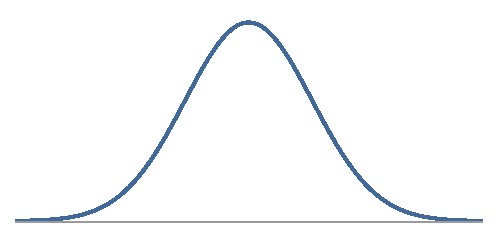
\includegraphics[width=0.7\textwidth]{\chpiv@path/4-1_normal_distribution/figures/simpleNormal/simpleNormal}
\end{center}

\end{frame}

%%%%%%%%%%%%%%%%%%%%%%%%%%%%%%%%%%%%

\begin{frame}
\frametitle{Normal distributions with different parameters}

\vspace{-0.5cm}
\begin{center}
$\mu$: mean, $\sigma$: standard deviation
\[N(\mu = 0, \sigma = 1) \hspace{1.4cm} N(\mu = 19, \sigma = 4) \]
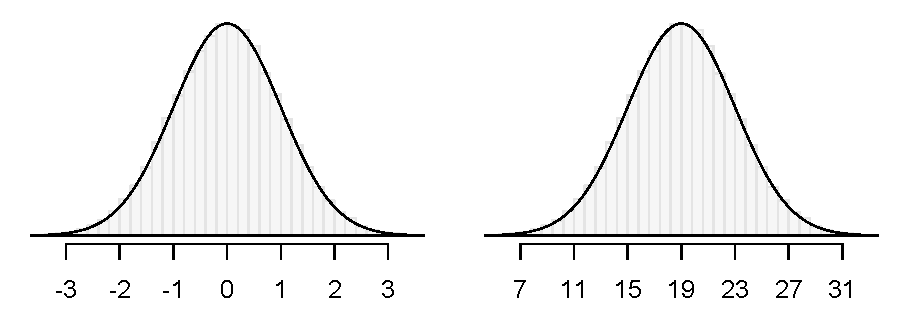
\includegraphics[width=0.6\textwidth]{\chpiv@path/4-1_normal_distribution/figures/twoSampleNormals/twoSampleNormals} \\
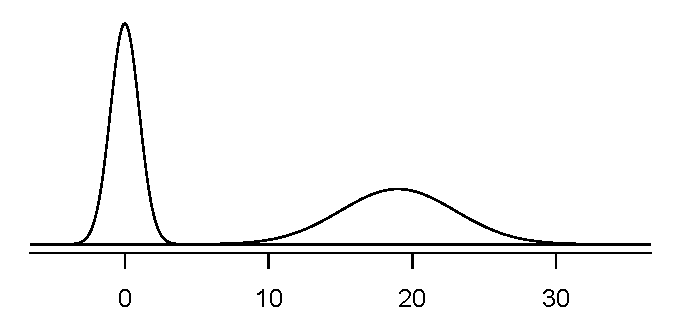
\includegraphics[width=0.6\textwidth]{\chpiv@path/4-1_normal_distribution/figures/twoSampleNormalsStacked/twoSampleNormalsStacked}
\end{center}

\end{frame}

\begin{frame}
\frametitle{Standardizing with Z scores}

\begin{itemize}

\item Z score of an observation is the number of standard deviations it falls above or below the mean.
\formula{\[Z = \frac{observation - mean}{SD}\]}
\pause

\item Z scores are defined for distributions of any shape, but only when the distribution is normal can we use Z scores to calculate percentiles.
\item If $X \sim N(\mu, \sigma)$, then $Z = \frac{X - \mu}{\sigma} \sim N(0, 1)$.

\pause
\item Observations that are more than 2 SD away from the mean ($|Z| > 2$) are usually considered unusual.

\end{itemize}

\end{frame}

%%%%%%%%%%%%%%%%%%%%%%%%%%%%%%%%%%%%

\begin{frame}
\frametitle{Percentiles}

\begin{itemize}

\item \hl{Percentile} is the percentage of observations that fall below a given data point. 

\item Graphically, percentile is the area below the probability distribution curve to the left of that observation.

\end{itemize}

\begin{center}
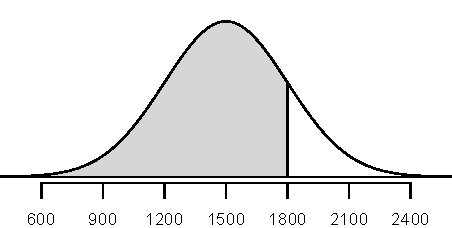
\includegraphics[width=0.7\textwidth]{\chpiv@path/4-1_normal_distribution/figures/satBelow1800/satBelow1800}
\end{center}

\end{frame}

\begin{frame}
\frametitle{Quality control}

\dq{{\small At Heinz ketchup factory the amounts which go into bottles of ketchup are supposed to be normally distributed with mean 36 oz. and standard deviation 0.11 oz. Once every 30 minutes a bottle is selected from the production line, and its contents are noted precisely. If the amount of ketchup in the bottle is below 35.8 oz. or above 36.2 oz., then the bottle fails the quality control inspection. What percent of bottles have less than 35.8 ounces of ketchup?}}

\soln{\pause
Let $X$ = amount of ketchup in a bottle: $X \sim N(\mu = 36, \sigma = 0.11)$ \\
\pause
\twocol{0.4}{0.6}{
\begin{center}
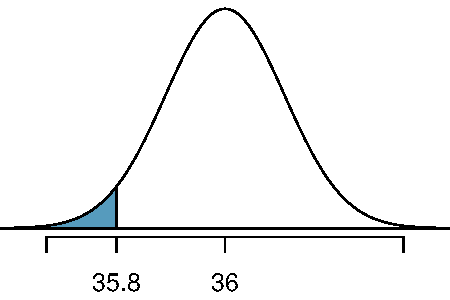
\includegraphics[width=\textwidth]{\chpiv@path/4-1_normal_distribution/figures/ketchup/ketchupLT358}
\end{center}
}
{
\pause
\vspace{2em}
\[ Z = \frac{35.8 - 36}{0.11} = -1.82 \]
\pause
\vspace{-1em}
\begin{eqnarray*}
    pnorm(-1.82)&=&0.03440\\
    pnorm(35.8,36,0.11)&=&0.03440
\end{eqnarray*}
}
}

\end{frame}

%%%%%%%%%%%%%%%%%%%%%%%%%%%%%%%%%%%%

\begin{frame}
\frametitle{Practice}

\pq{What percent of bottles \underline{pass} the quality control inspection?}

\vspace{-0.5cm}
\begin{multicols}{2}
\begin{enumerate}[(a)]
\item 1.82\%
\item 3.44\%
\item 6.88\%
\solnMult{93.12\%}
\item 96.56\%
\item[]
\end{enumerate}
\end{multicols}

\soln{
\vspace{-0.5cm}
\pause
\begin{columns}[c]
\column{0.3\textwidth}
\pause
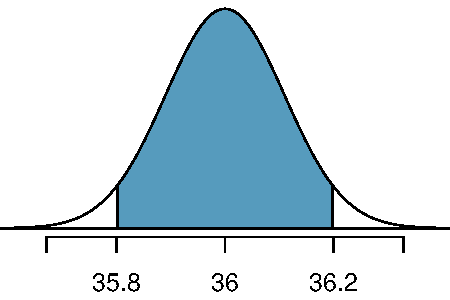
\includegraphics[width=\textwidth]{\chpiv@path/4-1_normal_distribution/figures/ketchup/ketchupBET}
\column{0.05\textwidth}
=
\pause
\column{0.3\textwidth}
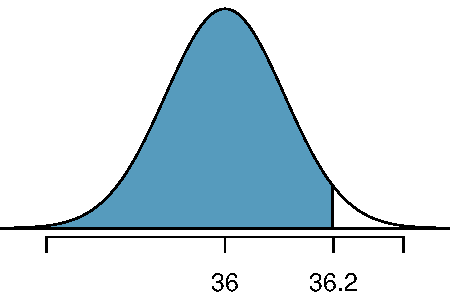
\includegraphics[width=\textwidth]{\chpiv@path/4-1_normal_distribution/figures/ketchup/ketchupLT362}
\column{0.05\textwidth}
-
\pause
\column{0.3\textwidth}
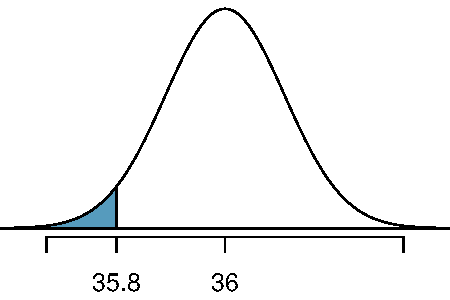
\includegraphics[width=\textwidth]{\chpiv@path/4-1_normal_distribution/figures/ketchup/ketchupLT358}
\end{columns}
\pause
% \begin{eqnarray*}
% Z_{35.8} = \frac{35.8 - 36}{0.11} = -1.82 \hspace{1.5cm}
% Z_{36.2} = \frac{36.2 - 36}{0.11} = 1.82 \\ \pause
% \end{eqnarray*}
\begin{small}
\begin{eqnarray*}
P(35.8 < X < 36.2) &=& pnorm(36.2, 35.8, 0.11) - pnorm(35.8, 36, 0.11) \\
&=& 0.9656 - 0.0344 = 0.9312 \\ \pause
P(-1.82 < Z < 1.82) &=& pnorm(-1.82) - pnorm(1.82) \\
&=& 0.9656 - 0.0344 = 0.9312
\end{eqnarray*}
\end{small}
}

\end{frame}

%%%%%%%%%%%%%%%%%%%%%%%%%%%%%%%%%%%%

\section{Edfinity Quiz}

%%%%%%%%%%%%%%%%%%%%%%%%%%%%%%%%%%%%

\begin{frame}[fragile]
\frametitle{Finding cutoff points}

\dq{Body temperatures of healthy humans are distributed nearly normally with mean 98.2$\degree$F and standard deviation 0.73$\degree$F. What is the cutoff for the lowest 3\% of human body temperatures?}

\pause

\twocol{0.3}{0.7}
{
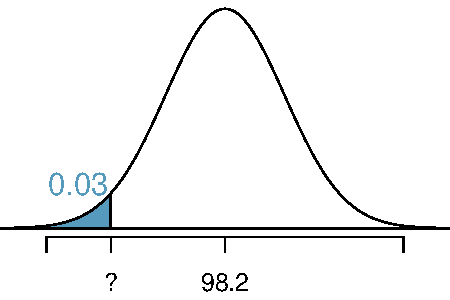
\includegraphics[width=\textwidth]{\chpiv@path/4-1_normal_distribution/figures/temp/tempLOW3PERC}
}
{
\pause
\begin{eqnarray*}
P(X < x) &=& 0.03 \rightarrow P(Z < \orange{-1.88}) = 0.03 \\ \pause
Z &=& \frac{obs~-~mean}{SD} \rightarrow \frac{x - 98.2}{0.73} = -1.88 \\ \pause
x &=& (-1.88 \times 0.73) + 98.2 = 96.8\degree F
\end{eqnarray*}
}
$\:$ \\
\begin{beamerboxesrounded}[shadow = true, lower = code body]{}
{\small \begin{verbatim}
> qnorm(0.03)
[1] -1.880794
\end{verbatim}
}
\end{beamerboxesrounded}

\ct{Mackowiak, Wasserman, and Levine (1992), \textit{A Critical Appraisal of 98.6 Degrees F, the Upper Limit of the Normal Body Temperature, and Other Legacies of Carl Reinhold August Wunderlick}.}

\end{frame}

%%%%%%%%%%%%%%%%%%%%%%%%%%%%%%%%%%%

\begin{frame}[fragile]
\frametitle{Practice}

\pq{Body temperatures of healthy humans are distributed nearly normally with mean 98.2$\degree$F and standard deviation 0.73$\degree$F. What is the cutoff for the highest 10\% of human body temperatures?}

\vspace{-0.5cm}
\begin{multicols}{2}
\begin{enumerate}[(a)]
\item 97.3$\degree$F
\solnMult{99.1$\degree$F}
\item 99.4$\degree$F
\item 99.6$\degree$F
\end{enumerate}
\end{multicols}

\soln{
\vspace{-0.5cm}
\pause
\vspace{-0.3cm}
\begin{center}
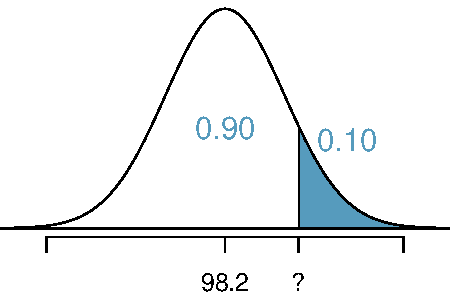
\includegraphics[width=0.3\textwidth]{\chpiv@path/4-1_normal_distribution/figures/temp/tempHIGH10PERC}
\end{center}
\vspace{-0.3cm}
\pause
\begin{small}
\begin{eqnarray*}
    P(X > x) = 0.10 &\rightarrow& P(X < x) = 0.90 \\
    &\rightarrow& x = qnorm(0.90, 98.2, 0.73) = 99.1\\ \pause
    P(Z<z) = 0.90 &\rightarrow& z = qnorm(0.90) = 1.28 \\
    &\rightarrow& x= (1.28 \times 0.73) + 98.2 = 99.1
\end{eqnarray*}
\end{small}
}

\end{frame}

%%%%%%%%%%%%%%%%%%%%%%%%%%%%%%%%%%%%

\section{R Demonstration: qnorm} 

%%%%%%%%%%%%%%%%%%%%%%%%%%%%%%%%%%%%

\section{Edfinity quiz: cutoff points}

%%%%%%%%%%%%%%%%%%%%%%%%%%%%%%%%%%%

\subsection{68-95-99.7 rule}

%%%%%%%%%%%%%%%%%%%%%%%%%%%%%%%%%%%%

\begin{frame}
\frametitle{68-95-99.7 Rule}

\begin{itemize}

\item For nearly normally distributed data, 
\begin{itemize}
\item about 68\% falls within 1 SD of the mean,
\item about 95\% falls within 2 SD of the mean,
\item about 99.7\% falls within 3 SD of the mean.
\end{itemize}

\item It is possible for observations to fall 4, 5, or more standard deviations away from the mean, but these occurrences are very rare if the data are nearly normal.

\end{itemize}

\begin{center}
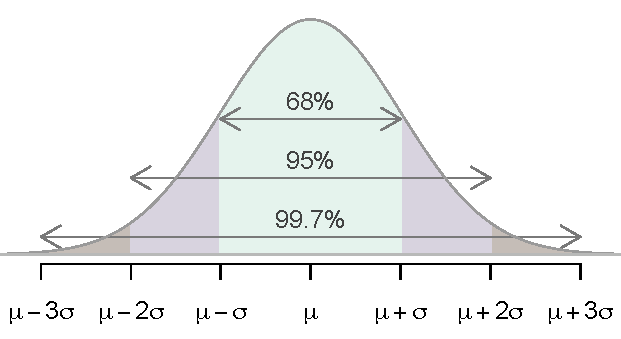
\includegraphics[width=0.7\textwidth]{\chpiv@path/4-1_normal_distribution/figures/6895997/6895997}
\end{center}

\end{frame}

%%%%%%%%%%%%%%%%%%%%%%%%%%%%%%%%%%%%

\begin{frame}
\frametitle{Describing variability using the 68-95-99.7 Rule}

SAT scores are distributed nearly normally with mean 1500 and standard deviation 300.

\pause
\begin{itemize}

\item $\sim$68\% of students score between 1200 and 1800 on the SAT. 

\item $\sim$95\% of students score between 900 and 2100 on the SAT. 

\item $\sim$99.7\% of students score between 600 and 2400 on the SAT. 

\end{itemize}

\begin{center}
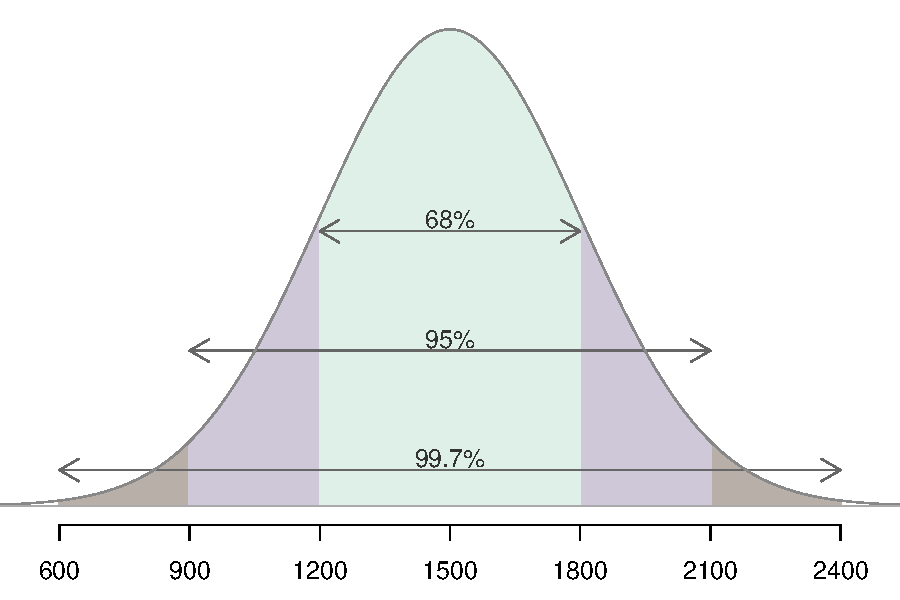
\includegraphics[width=0.65\textwidth]{\chpiv@path/4-1_normal_distribution/figures/sat_empirical/sat_empirical}
\end{center}

\end{frame}

%%%%%%%%%%%%%%%%%%%%%%%%%%%%%%%%%%%%

\section{Edfinity quiz: Geometric logic}  

%%%%%%%%%%%%%%%%%%%%%%%%%%%%%%%%%%%%

\begin{frame}[fragile]
\frametitle{Number of hours of sleep on school nights}

\only<1 | handout:0>{
\begin{center}
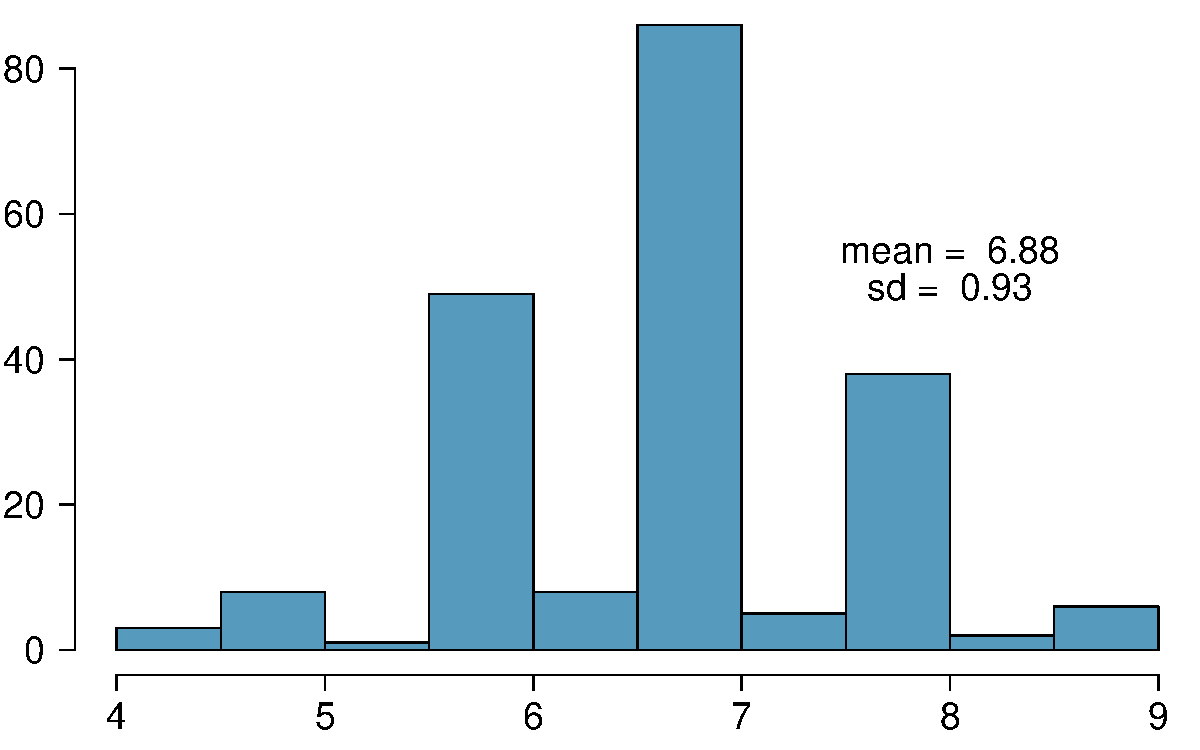
\includegraphics[width=0.75\textwidth]{\chpiv@path/4-1_normal_distribution/figures/sleep/sleep-hist} 
\end{center}
\vspace{-0.25cm}
\begin{itemize}
\item Mean = 6.88 hours, SD = 0.92 hrs
\item[] \textcolor{white}{72\% of the data are within 1 SD of the mean: $6.88 \pm 0.93$}
\item[] \textcolor{white}{92\% of the data are within 2 SD of the mean: $6.88 \pm 2 \times 0.93$}
\item[] \textcolor{white}{99\% of the data are within 3 SD of the mean: $6.88 \pm 3 \times 0.93$}
\end{itemize}
}

\only<2 | handout:0>{
\begin{center}
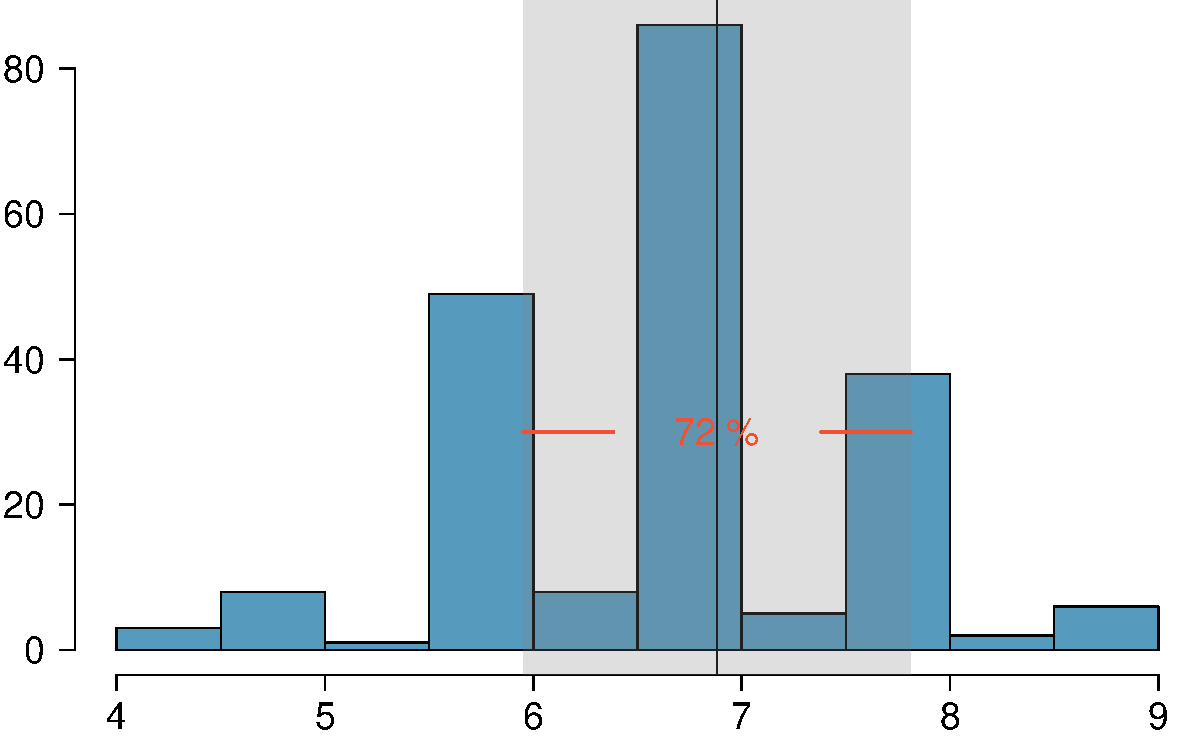
\includegraphics[width=0.75\textwidth]{\chpiv@path/4-1_normal_distribution/figures/sleep/sleep-hist-sd1} 
\end{center}
\vspace{-0.25cm}
\begin{itemize}
\item Mean = 6.88 hours, SD = 0.92 hrs
\item 72\% of the data are within 1 SD of the mean: $6.88 \pm 0.93$
\item[] \textcolor{white}{92\% of the data are within 2 SD of the mean: $6.88 \pm 2 \times 0.93$}
\item[] \textcolor{white}{99\% of the data are within 3 SD of the mean: $6.88 \pm 3 \times 0.93$}
\end{itemize}
}

\only<3 | handout:0>{
\begin{center}
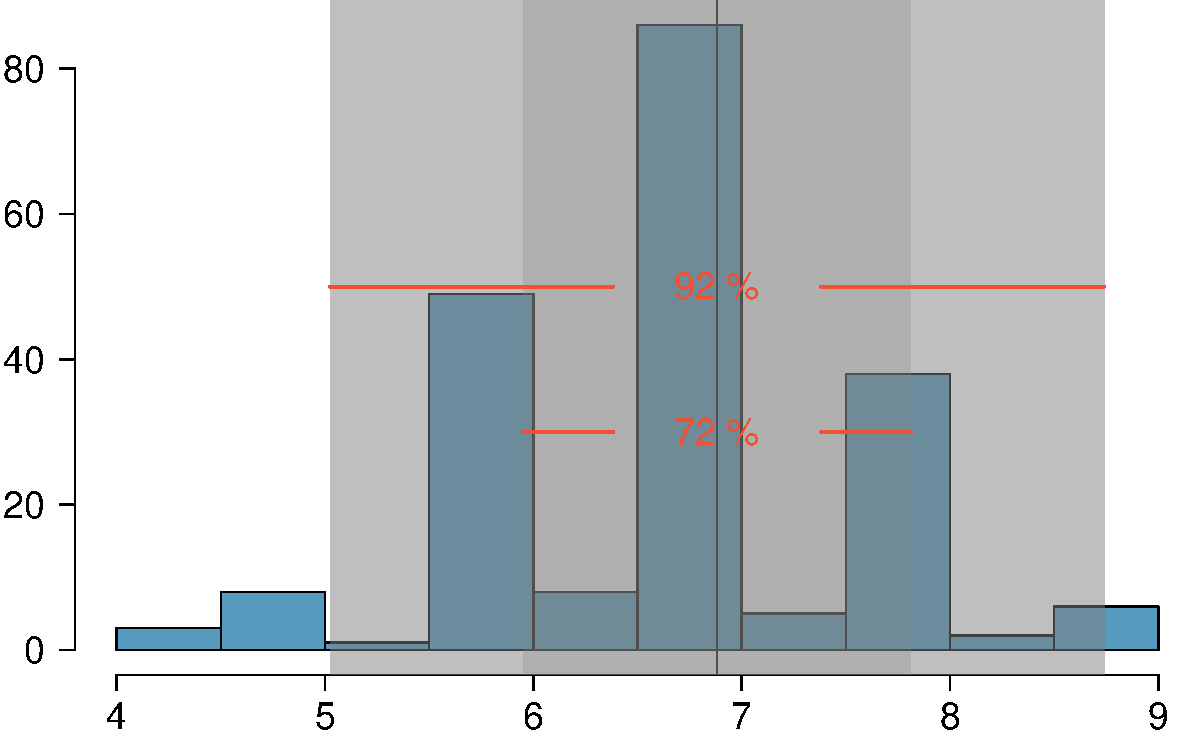
\includegraphics[width=0.75\textwidth]{\chpiv@path/4-1_normal_distribution/figures/sleep/sleep-hist-sd2} 
\end{center}
\vspace{-0.25cm}
\begin{itemize}
\item Mean = 6.88 hours, SD = 0.92 hrs
\item 72\% of the data are within 1 SD of the mean: $6.88 \pm 0.93$
\item 92\% of the data are within 1 SD of the mean: $6.88 \pm 2 \times 0.93$
\item[] \textcolor{white}{99\% of the data are within 3 SD of the mean: $6.88 \pm 3 \times 0.93$}
\end{itemize}
}

\only<4>{
\begin{center}
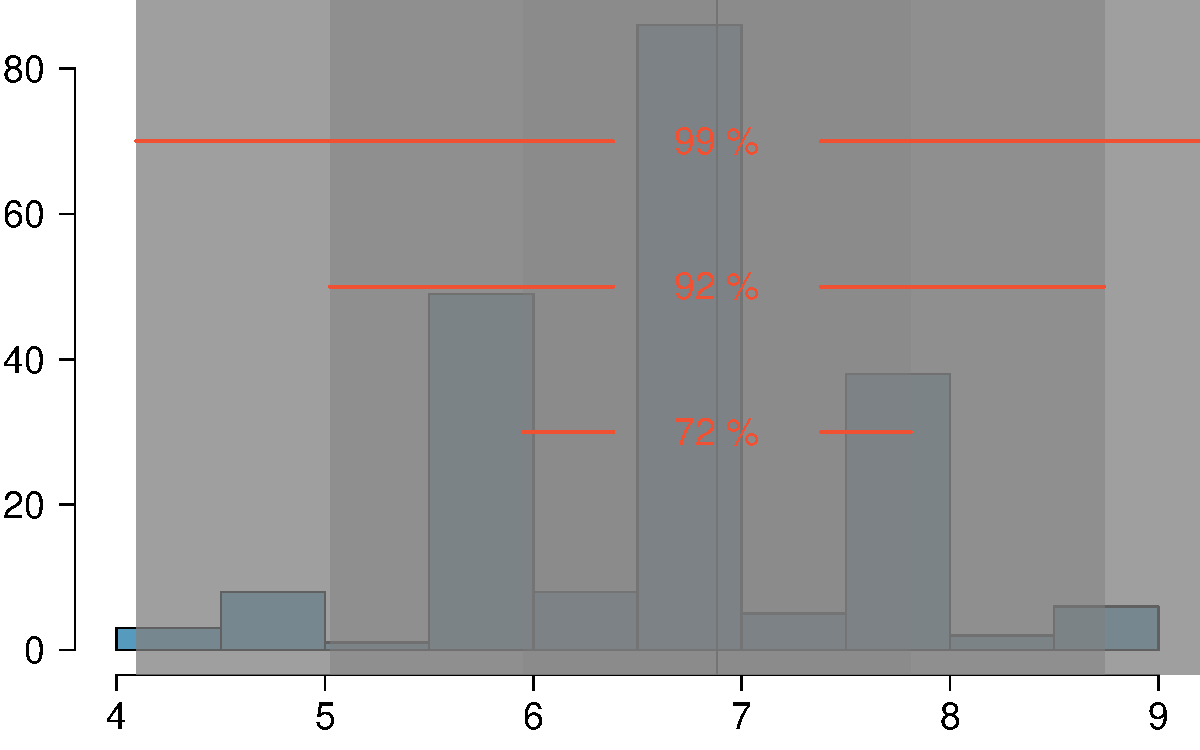
\includegraphics[width=0.75\textwidth]{\chpiv@path/4-1_normal_distribution/figures/sleep/sleep-hist-sd3} 
\end{center}
\vspace{-0.25cm}
\begin{itemize}
\item Mean = 6.88 hours, SD = 0.92 hrs
\item 72\% of the data are within 1 SD of the mean: $6.88 \pm 0.93$
\item 92\% of the data are within 2 SD of the mean: $6.88 \pm 2 \times 0.93$
\item 99\% of the data are within 3 SD of the mean: $6.88 \pm 3 \times 0.93$
\end{itemize}
}

\end{frame}

%%%%%%%%%%%%%%%%%%%%%%%%%%%%%%%%%%%%

% \begin{frame}
% \frametitle{Practice}

% \pq{Which of the following is \underline{false}?}

% \begin{enumerate}[(a)]
% \item Majority of Z scores in a right skewed distribution are negative.
% \solnMult{In skewed distributions the Z score of the mean might be different than 0.}
% \item For a normal distribution, IQR is less than $2 \times SD$.
% \item Z scores are helpful for determining how unusual a data point is compared to the rest of the data in the distribution.
% \end{enumerate}

% \end{frame}

%%%%%%%%%%%%%%%%%%%%%%%%%%%%%%%%%%%%

% \section{R Demonstration: Variability with 68-95-99.7 rule}

%%%%%%%%%%%%%%%%%%%%%%%%%%%%%%%%%%%%

% \section{Edfinity quiz: Variability, concept review}
% Thinking like the last Practice slide, commented out above  
% ES: Make it into a think/pair/share?

%%%%%%%%%%%%%%%%%%%%%%%%%%%%%%%%%%%%
% End document
%%%%%%%%%%%%%%%%%%%%%%%%%%%%%%%%%%%%

\end{document}